\documentclass[12pt]{article}
\usepackage{sbc-template}
\usepackage[T1]{fontenc}
\usepackage[utf8]{inputenc}
\usepackage[brazil]{babel}
\usepackage{graphicx}
\usepackage[hidelinks]{hyperref}

\title{Locadora de veículos\\Integração do front-end com a API}
\author{Esther Caldeira Rivadalves\inst{1}}
\address{Análise e Desenvolvimento de Sistemas -- PUC Minas\\Campus São Gabriel}

\begin{document}
\maketitle
\section{Problema da locadora}
A operação de uma locadora precisa relacionar seus veículos e clientes a cada aluguel. O sistema permite registrar a retirada, acompanhar a previsão e concluir a devolução. A interface centraliza os cadastros e disponibiliza consultas para acompanhar a frota e o faturamento.

\section{Modelagem e integração}
Na modelagem relacional, um fabricante e uma categoria podem estar associados a vários veículos. Cada aluguel vincula um cliente a um veículo. O SQL Server armazena os registros, e as chaves estrangeiras preservam os vínculos. A aplicação ASP.NET Core consulta o banco por meio do Entity Framework Core e fornece os resultados em JSON. O front-end usa HTML, CSS, Bootstrap e JavaScript para chamar as rotas HTTP.

\begin{figure}[ht]
\centering
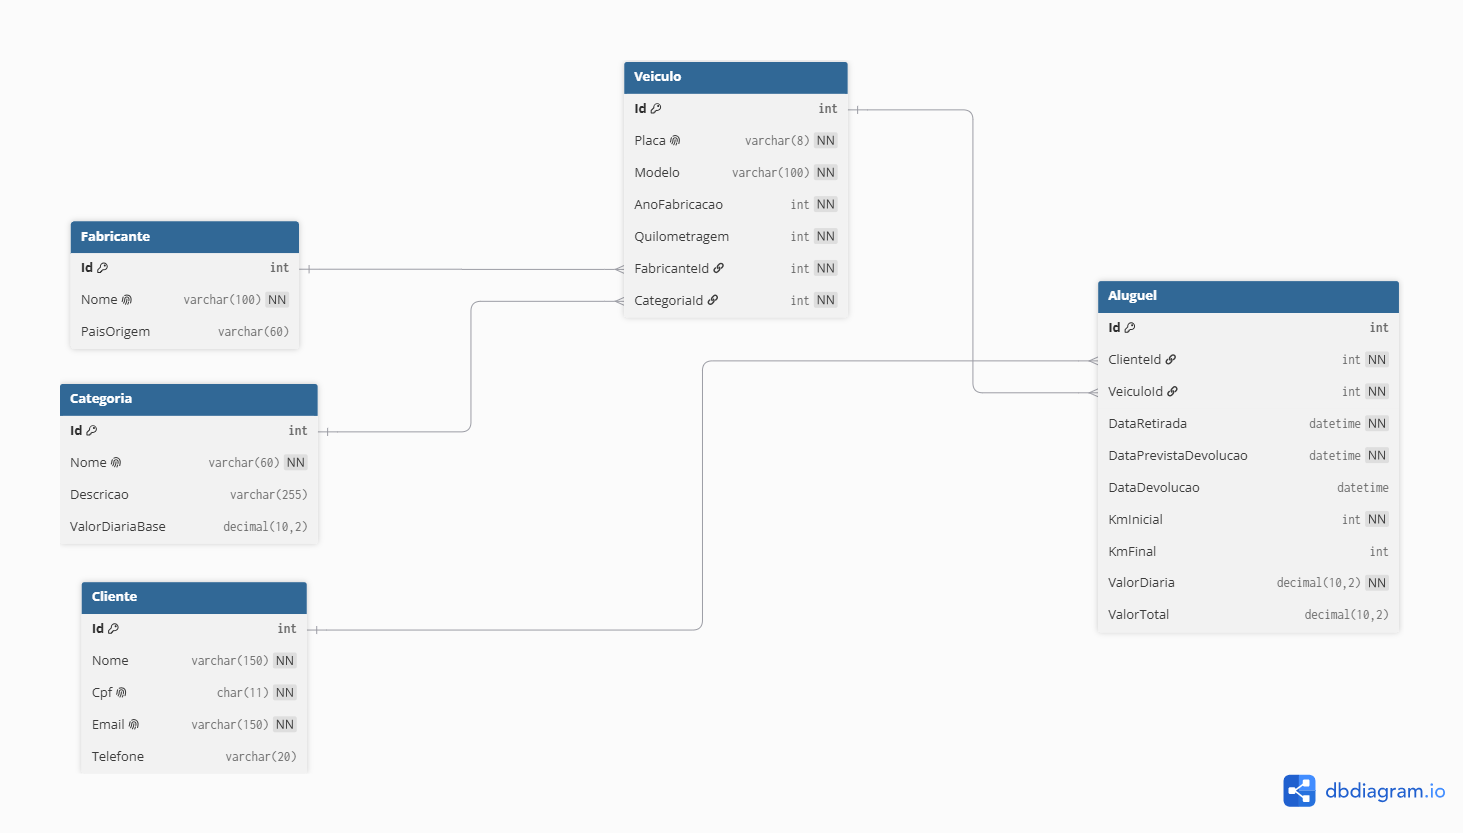
\includegraphics[width=.93\linewidth]{../Evidencias-Etapa1/dbdiagram.io.png}
\caption{Diagrama da modelagem relacional produzida na primeira parte.}
\end{figure}

\section{Artefatos da entrega}
O código está na pasta \texttt{frontend/}. Os \href{https://github.com/esthercr0/Locadora/tree/frontend/etapa-1/Docs/Wireframes}{wireframes navegáveis} estão em \texttt{Docs/Wireframes/index.html} e podem ser abertos no navegador após baixar o arquivo. Cada cadastro permite consultar, incluir, editar e excluir registros conforme as regras da API. Fabricantes têm busca por nome e país, categorias por nome e faixa de diária, veículos por modelo e placa, clientes por nome e CPF, e aluguéis por cliente e placa. Na devolução, a API calcula o total e atualiza a quilometragem do veículo.

\section{Consultas da primeira parte}
\begin{itemize}
\item \textbf{Veículos por fabricante}. \nolinkurl{GET /api/veiculos/por-fabricante/{id}} retorna os veículos vinculados ao fabricante escolhido.
\item \textbf{Veículos disponíveis}. \nolinkurl{GET /api/veiculos/disponiveis} seleciona no banco os veículos sem aluguel aberto. A interface permite restringir a consulta por categoria e exibe placa, modelo, fabricante e categoria.
\item \textbf{Clientes sem aluguel ativo}. \nolinkurl{GET /api/clientes/sem-aluguel-ativo} retorna clientes sem locação em aberto.
\item \textbf{Aluguéis por período}. \nolinkurl{GET /api/alugueis/por-periodo} filtra pela data de retirada com os parâmetros \texttt{inicio} e \texttt{fim}.
\item \textbf{Faturamento por categoria}. \nolinkurl{GET /api/alugueis/faturamento-por-categoria} agrega aluguéis finalizados e apresenta quantidade de locações e valor total por categoria.
\end{itemize}

\section{Validação}
Os cadastros de Honda e Hyundai feitos na interface foram confirmados com consulta direta à tabela de fabricantes no SQL Server. Também foram confirmados o filtro de fabricantes e a edição e exclusão de categorias. Os testes automatizados do cliente HTTP foram executados. A validação das cinco consultas com o banco local deve ser demonstrada na gravação.

\end{document}
